\documentclass{beamer}
\usetheme{metropolis}
\usepackage{graphicx}
\defbeamertemplate*{title page}{customized}[1][]
{
  \usebeamercolor[fg]{titlegraphic}\inserttitlegraphic
  \begin{center}
    \usebeamerfont{title}\inserttitle\par
    \usebeamerfont{subtitle}\usebeamercolor[fg]{subtitle}\insertsubtitle\par
    \bigskip
    \usebeamerfont{author}\insertauthor\par
    \usebeamerfont{institute}\insertinstitute\par
    \usebeamerfont{date}\insertdate\par
  \end{center}
}

\title{Unrolling Recurrent Neural Networks}
\author{Petru Rebeja}
\titlegraphic{
  \begin{center}
    
\includegraphics[width=0.4\textwidth]{../img/iasi-ai-logo.png}
  \end{center}
}
% \logo{
\includegraphics[height=1.5cm]{../img/iasi-ai-logo.png}}
\begin{document}
\maketitle
\begin{frame}
  \frametitle{The shortcomings of a traditional Neural Network \cite{rnn-efectiveness}}
  \begin{columns}
    \begin{column}{0.3\textwidth}
      \begin{center}
        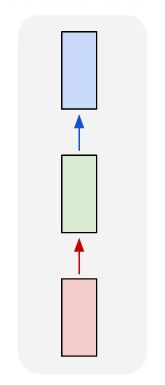
\includegraphics[height=0.7\textheight]{../img/vanilla-nn.png}
      \end{center}
    \end{column}
    \begin{column}{0.7\textwidth}
      \begin{itemize}
        \item Constrained to a \textbf{fixed size input} and produce \textbf{fixed size output}.
        \item The number of \textbf{computational steps} is \textbf{fixed}.
      \end{itemize}
    \end{column}
  \end{columns}
\end{frame}
\begin{frame}
  \frametitle{Recurrent Neural Networks}
  \begin{itemize}
    \item Are specialized for processing a sequence of values \cite{goodfellow-et-al-2016}
    \item As convolutional networks can scale to images of variable size, recurrent networks can process sequences of variable length \cite{goodfellow-et-al-2016}
    \item Offer a more powerful way of processing the data \cite{rnn-lecture} and are Turing-Complete \cite{siegelmann1995}
    \item Are a special case of \textbf{Recursive Neural Networks} which, in turn, are a separate topic (maybe for another presentation).
  \end{itemize}
\end{frame}
\begin{frame}[allowframebreaks]
  \frametitle{Flavors of Recurrent Networks \cite{rnn-efectiveness}}
  \begin{columns}
    \begin{column}{0.3\textwidth}
      \begin{center}
        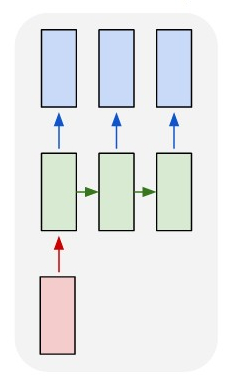
\includegraphics[height=0.7\textheight]{../img/rnn-one-to-many.png}
      \end{center}
    \end{column}
    \begin{column}{0.7\textwidth}
      \begin{center}
        \textbf{One to many}
      \end{center}
      \begin{itemize}
        \item Given a fixed size input, the network outputs a sequence of values.
        \item e.g. \textit{Image captioning} - The network takes an image and outputs a sequence of words.
      \end{itemize}
    \end{column}
  \end{columns}
  \framebreak
  \begin{columns}
    \begin{column}{0.3\textwidth}
      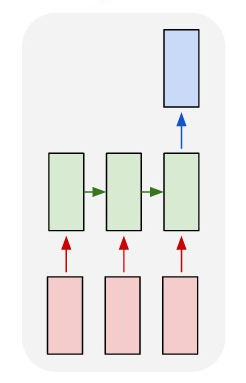
\includegraphics[height=0.7\textheight]{../img/rnn-many-to-one.png}
    \end{column}
    \begin{column}{0.7\textwidth}
      \begin{center}
        \textbf{Many to one}
      \end{center}
      \begin{itemize}
        \item Given a sequence of values, the network outputs a fixed size result.
        \item e.g. \textit{Sentiment analysis} - The network takes a sentence (sequence of words) and classifies it as expressing positive, negative or neutral sentiment.
      \end{itemize}
    \end{column}
  \end{columns}
  \framebreak
  \begin{columns}
    \begin{column}{0.5\textwidth}
      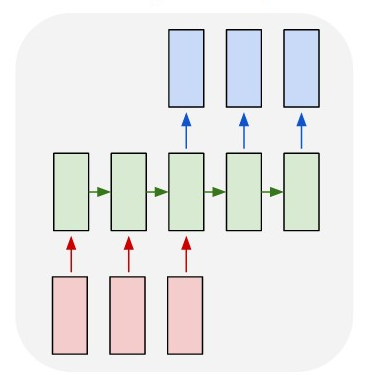
\includegraphics[height=0.7\textheight]{../img/rnn-many-to-many-1.png}
    \end{column}
    \begin{column}{0.5\textwidth}
      \begin{center}
        \textbf{Many to many (I)}
      \end{center}
      \begin{itemize}
        \item Given a sequence of values, the network outputs another sequence of values.
        \item e.g. \textit{Machine translation} - The network takes a sentence in English and then outputs a sentence in Romanian.
      \end{itemize}
    \end{column}
  \end{columns}
  \framebreak
  \begin{columns}
    \begin{column}{0.3\textwidth}
      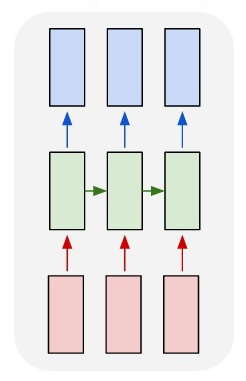
\includegraphics[height=0.7\textheight]{../img/rnn-many-to-many-2.png}
    \end{column}
    \begin{column}{0.7\textwidth}
      \begin{center}
        \textbf{Many to many (II)}
      \end{center}
      \begin{itemize}
        \item Given a sequence of values, the network outputs another sequence of values.
        \item e.g. \textit{Video classification on frame level} - The network takes a sequence of video frames and classifies each one based on frame contents \textit{and} the frames before.
      \end{itemize}
    \end{column}
  \end{columns}
\end{frame}
\begin{frame}[allowframebreaks]
  \frametitle{References}
  \bibliographystyle{amsalpha}
  \bibliography{unrolling-rnns}
\end{frame}
\end{document}
%%% Local Variables:
%%% mode: latex
%%% TeX-master: t
%%% End:
